\documentclass{beamer}
\usetheme[titleformat=smallcaps,numbering=fraction,block=fill]{metropolis}
\IfFileExists{fonts.tex}{\input{fonts.tex}}{} % for small caps @ overleaf

\usepackage{amsmath,amssymb,amsthm,graphicx,multirow}
\usepackage[center]{caption}
\usepackage{subfig}
\usepackage{appendixnumberbeamer,booktabs}

\everymath{\displaystyle}
\newtheorem{proposition}{Proposition}
\newcommand{\E}{\mathop{{}\mathbb{E}}}
\newcommand{\floor}[1]{{\left\lfloor{#1}\right\rfloor}}
\newcommand{\ceil}[1]{{\left\lceil{#1}\right\rceil}}
\DeclareMathOperator*{\vol}{vol}
\DeclareMathOperator*{\Vol}{Vol}
\DeclareMathOperator*{\dist}{dist}

\renewcommand{\appendixname}{{Appendix}} % fix warning
\newcommand{\autotitle}{\secname\ifdefempty{\subsecname}{}{~--- \subsecname}}
\newcommand{\clearsubsecname}{\long\def\subsecname{}}
\newcommand{\vtable}[2][c]{% \vtable[<col align>]{<stuff>}
    \renewcommand{\arraystretch}{0.8}%
    \begin{tabular}[c]{@{}#1@{}}#2\end{tabular}}
\newcommand{\smalldisplayskips}{
    \setlength{\abovedisplayskip}{3pt}
    \setlength{\belowdisplayskip}{3pt}}
\newcommand{\normaldisplayskips}{
    \setlength{\abovedisplayskip}{8pt}
    \setlength{\belowdisplayskip}{8pt}}
%\setbeamerfont{bibliography entry author}{size=\footnotesize}
%\setbeamerfont{bibliography entry title}{size=\footnotesize}
%\setbeamerfont{bibliography entry location}{size=\footnotesize}

%%%%%%%%%%%%%%%%%%%%%%%%%%%%%%%%%%%%%%%%%%%%%%%%%%%%%%%%%%%%%%%%%%%%%%%%%%%%%%%%

\title{Expanders in Power Law Graphs}
\author{Anton Cherniavskyi}
\date{October 22, 2018}
\institute{Simon Fraser University}
\titlegraphic{\hfill
\includegraphics[scale=0.08]{images/sfu_logo}}

%%%%%%%%%%%%%%%%%%%%%%%%%%%%%%%%%%%%%%%%%%%%%%%%%%%%%%%%%%%%%%%%%%%%%%%%%%%%%%%%

\begin{document}

\maketitle

\section{Introduction}
\clearsubsecname

\begin{frame}{\autotitle}
    \textbf{A power law} is a relation of the form $f(x)=ax^b$.
    \begin{figure}
        \centering
        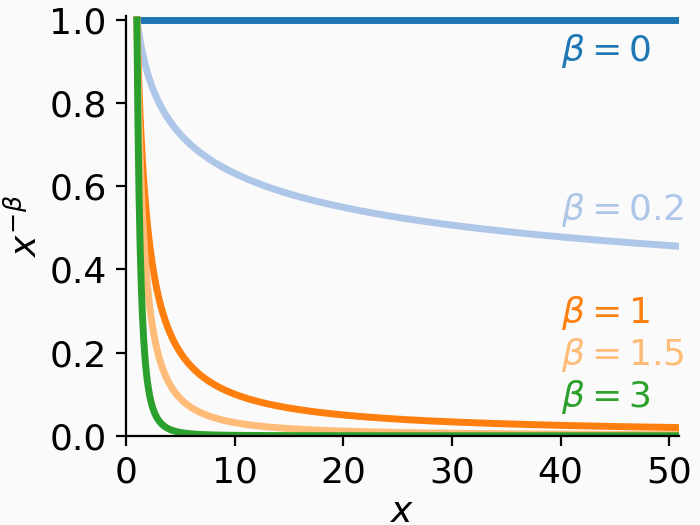
\includegraphics[scale=0.5]{images/generated_presentation/power-law}
        \caption{Power law functions}
    \end{figure}
    \begin{exampleblock}{Examples}
        Pareto principle, population of cities,
        magnitude of earthquakes, and preferential attachment processes.
    \end{exampleblock}
\end{frame}

\begin{frame}{\autotitle}
    \textbf{Power-law graphs} have either degrees,
    or the number of vertices with a given degree
    proportional to a power law $x^{-\beta}$, for some constant $\beta\geq0$.
    \begin{figure}
        \centering
        \subfloat{{
            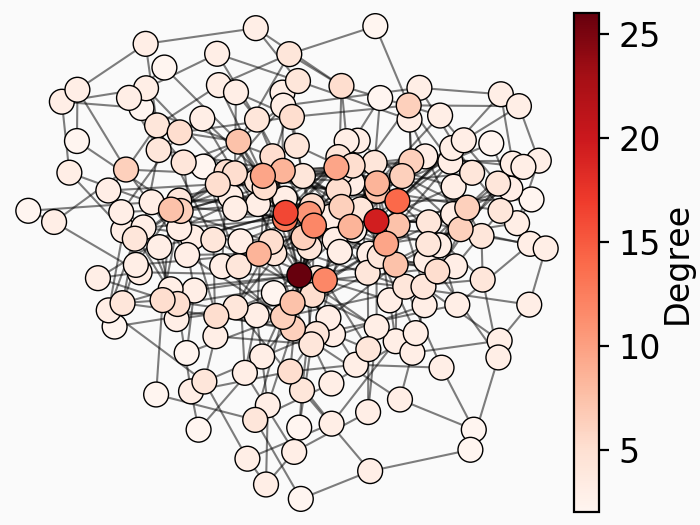
\includegraphics[scale=0.5]
            {images/generated_presentation/power-law-graph}
        }}
        \qquad
        \subfloat{{
            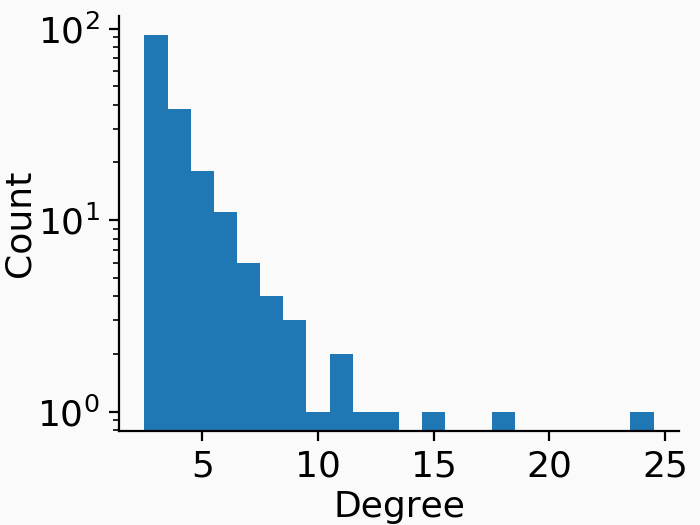
\includegraphics[scale=0.5]
            {images/generated_presentation/power-law-deg-distribution}
        }}
        \caption{Example of a power-law graph and its degree distribution,
            $n=200$~vertices, $\deg(i)=n^{0.6}/i^{0.4}$}
    \end{figure}
\end{frame}

\begin{frame}{\autotitle}
    \textbf{Expanders} are ``well-connected'' graphs that are extensively used
    in computing science for purposes like
    \begin{itemize}
        \item decomposition of graphs
        \item designing of the routing schemes
        \item graph exploration
        \item proving SAT lower bounds and the PCP theorem, etc.
    \end{itemize}
    \begin{figure}
        \centering
        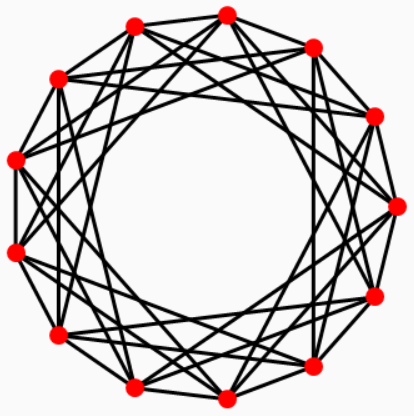
\includegraphics[scale=0.3]{images/paley_grey}
        \caption{Paley graph is an expander}
    \end{figure}
\end{frame}

\subsection{Related Work}

\begin{frame}{\autotitle}
    \begin{description}
        \item[\cite{acl01}] the model of random power-law graphs with
        the exact frequencies of degrees,
        connectivity and sizes of the connected components.
        
        \item[\cite{gms03}] $\Theta(1)$ conductance of random power-law graphs
        with $2<\beta<3$, degrees between $3$ and $O\left(\sqrt{n}\right)$,
        and volume $O(n)$.
        
        \item[\cite{cl04}] the average distance in random graphs
        with given expected degree sequences,
        the ``octopus'' graph and its $O(\log n)$ diameter.
        
        \item[\cite{kri17}] a linear size expanders in ``locally sparse'' graphs
        and in $G(n,p)$ graphs, including constructive proof.
    \end{description}
\end{frame}

\begin{frame}{\autotitle}
    \small
    \begin{table}
        \caption{Comparison of power-law graph models}
        \begin{tabular}{@{} lll @{}}
            \toprule
            Model & Object & Definition\\
            \midrule
            Model from~\cite{acl01} & \vtable[l]{exact\\frequencies}
                & $|\{i \in V\;|\;\deg(i)=x\}|=\frac{e^\alpha}{x^\beta}$\\[10pt]
            Coin toss model & \vtable[l]{expected\\frequencies}
                & $\E_G[|\{i\in V\;|\;\deg(i)=x\}|]=\frac{e^\alpha}{x^\beta}$\\[10pt]
            \vtable[l]{The ``octopus'' graphs\\from~\cite{cl04}} & \vtable[l]{expected\\degrees}
                & $\E_G[\deg(i)]=ci^{-1/(\beta-1)}$\\[10pt]
            Permutation model & \vtable[l]{exact\\degrees}
                & $\deg(i)=\frac{pn}{i^\beta}$\\
            \bottomrule
        \end{tabular}
    \end{table}
\end{frame}

\begin{frame}{\autotitle}
    \footnotesize
    \begin{table}
        \caption{Consistency of sizes between different results}
        \begin{tabular}{@{} l|c|c|c|c @{}}
            \specialrule{\heavyrulewidth}{0pt}{0pt}
            & \multicolumn{4}{c}{$\beta$}\rule{0pt}{13pt}\\[3pt]
            \cline{2-5}
            & $(0;1.6]$ & $(1.6;1.72]$ & $(1.72;3.48)$ & $(3.48;\infty)$\rule{0pt}{13pt}\\[3pt]
            \hline
            \vtable[l]{The largest components\\in graphs from~\cite{acl01}}
                & \multicolumn{3}{|c|}{the giant component, $\Theta(n)$}
                & $O\left(n^{2/\beta}\log n\right)$\rule{0pt}{17pt}\\[7pt]
            \hline
            \vtable[l]{Our edge expanders\\in coin toss model}
                & $\Theta(n)$
                & \multicolumn{3}{|c}{$\Theta\left(n^{1/\beta}\right)$}\rule{0pt}{17pt}\\[7pt]
            \hline
            \vtable[l]{Vertex \& edge expanders\\in $G(n,p)$ by~\cite{kri17}}
                & \multicolumn{4}{|c}{$\Theta(n)$}\rule{0pt}{17pt}\\[7pt]
            \hline
            \vtable[l]{Our edge expanders\\in permutation model}
                & \multicolumn{2}{|c|}{$\Theta(n)$}
                & \multicolumn{2}{|c}{---}\rule{0pt}{17pt}\\[7pt]
            \specialrule{\heavyrulewidth}{0pt}{0pt}
        \end{tabular}
    \end{table}
\end{frame}

\section{Preliminaries}
\clearsubsecname

\subsection{The Sum of a Special Series}

\begin{frame}{\autotitle}
    Multiple proofs are reduced to upper-bounding the sum $S_n$,
    for~$n\to\infty$ and some constants $0<\alpha\leq 1/2$, $c_1>0$, and $c_2>0$:
    \begin{equation*}
        S_n=\sum_{s=1}^{\alpha n}{\left(c_1(s/n)^{c_2}\right)^s}
    \end{equation*}
    
    \begin{proposition}
        \begin{enumerate}
            \item $S_n<1$, if $c_2\geq1+\log c_1$.
            \item $S_n\leq o(1)$, for some sufficiently small $\alpha$.
            \item $S_n\leq o(1)$, for any $\alpha\leq 1/2$ if $c_2>\max\{1,\log c_1\}$.
            Moreover, $c_1$ and $c_2$ can be superconstants in terms of $n$,
            as long as $c_1=o\left(n^{c_2-1}\right)$.
        \end{enumerate}
    \end{proposition}
\end{frame}

\subsection{Generalized Harmonic Numbers}

\begin{frame}{\autotitle}
    \textbf{Riemann zeta function} is defined for $s\in\mathbb{C}$ with $\Re(s)>1$:
    \begin{equation*}
        \zeta(s)=\sum_{k=1}^{\infty}\frac{1}{k^s}
    \end{equation*}
    \only<1>{
        \leavevmode
        \begin{figure}
            \centering
            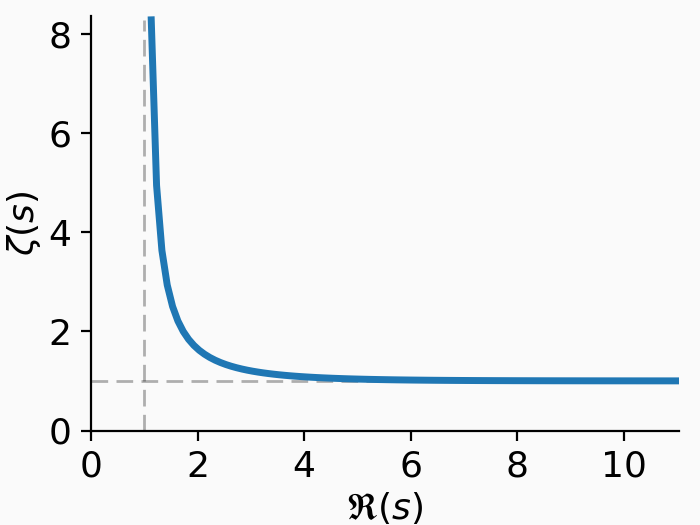
\includegraphics[scale=0.5]{images/generated_presentation/zeta}
            \caption{Riemann zeta function for $s\in\mathbb{C}$\\
                with $\Re(s)>1$ and $\Im(s)=0$}
        \end{figure}
    }
    
    \only<2->{
        \textbf{Generalized harmonic number:}
        \begin{equation*}
            H_{n,\beta}=\sum_{k=1}^{n}\frac{1}{k^\beta}\approx
            \begin{cases}
                \frac{n^{1-\beta}}{1-\beta} & \quad \text{if } \beta<1,\\
                \ln n & \quad \text{if } \beta=1,\\
                \zeta(\beta) & \quad \text{if } \beta>1.
            \end{cases}
        \end{equation*}
        
        For $\beta>1$ as $n\to\infty$, applying the Euler-Maclaurin formula:
        \begin{equation*}
            H_{n,\beta}=\zeta(\beta)-\frac{1}{(\beta-1)n^{\beta-1}}
            -\frac{1}{2n^\beta}-O\left(\frac{1}{n^{\beta+1}}\right)
            =\zeta(\beta)-o(1)
        \end{equation*}
    }
\end{frame}

\subsection{Uniform Random Graphs}

\begin{frame}{\autotitle}
    The most commonly used models of uniform random graphs are $G(n,p)$
    and $G(n,m)$ introduced by Gilbert and by Erd\H{o}s and R\'enyi in 1959.
    
    Let $N=\binom{n}{2}$ be the maximum number of edges.
    \begin{description}
        \item[$G(n,p)$] is a graph with $\Pr_G[(i,j)\in E]=p$, for any $i,j\in V$.
        \item[$G(n,m)$] is a graph with exactly $m$ edges,
        and each of $\binom{N}{m}$ graphs is chosen uniformly at random.
    \end{description}
    If $m=pN$ and $p>\frac{\log n}{n}$ as $n\to\infty$,
    then $G(n,p)$ and $G(n,m)$ are almost identical.
\end{frame}

\begin{frame}{\autotitle}
    \begin{table}
        \caption{The behavior of $G(n,p)$}
        \begin{tabular}{@{} llr @{}}
            \toprule
            \multicolumn{2}{@{} l}{Regime} & Property\\
            \midrule
            \multicolumn{2}{@{} l}{$p=o(1/n)$} & the graph is a disjoint union of trees\\[5pt]
            & $c<1$ & the largest component is $O(\log n)$\\
            $p=c/n$ & $c=1$ & the largest component is $\Theta\left(n^{2/3}\right)$\\
            & $c>1$ & a unique giant component of size $\Theta(n)$\\[5pt]
            \multicolumn{2}{@{}l}{$p<(1-\epsilon)\log n/n$} & the graph is disconnected w.h.p.\\
            \multicolumn{2}{@{}l}{$p>(1+\epsilon)\log n/n$} & the graph is connected w.h.p.\\
            \bottomrule
        \end{tabular}
    \end{table}
\end{frame}

\subsection{Expander Graphs}

\begin{frame}{\autotitle}
    \smalldisplayskips
    For any non-empty $S\subset V$ in $G=(V,E)$, the size of a cut $(S,V\backslash S)$:
    \begin{equation*}
        \partial S=e(S,V\backslash S)=\{(u,v)\in E\;|\;u\in S,v\in V\backslash S\},
    \end{equation*}
    and the external neighborhood of $S$ in $G$:
    \begin{equation*}
        N_G(S)=\{v\in V\backslash S\;|\;\exists u\in S\,((u,v)\in E)\}.
    \end{equation*}
    \normaldisplayskips
    
    \begin{columns}[T,onlytextwidth]
        \column{0.5\textwidth}
        \textbf{$(\alpha n,\gamma)$ edge expander} is a graph
        that for some $\alpha\leq 1/2$ and $\gamma>0$ satisfies:
        \begin{equation*}
            \min_{\substack{S\subset V\\0<|S|\leq\alpha n}}\frac{|\partial S|}{|S|}\geq\gamma
        \end{equation*}
        
        \column{0.5\textwidth}
        \textbf{$(\alpha n,\gamma)$ vertex expander} is a graph
        that for some $\alpha\leq 1/2$ and $\gamma>0$ satisfies:
        \begin{equation*}
            \min_{\substack{S\subset V\\0<|S|\leq\alpha n}}\frac{|N_G(S)|}{|S|}\geq\gamma
        \end{equation*}
    \end{columns}
\end{frame}

\begin{frame}{\autotitle}
    \textbf{The Cheeger constant} is simply edge expansion when $\alpha=1/2$:
    \begin{equation*}
        h(G)=\min_{\substack{S\subset V\\0<|S|\leq n/2}}\frac{|\partial S|}{|S|}
    \end{equation*}
    
    If the Laplacian $L$ of $G$ has eigenvalues
    $0=\lambda_1 \leq \lambda_2 \leq \dots \leq \lambda_{n}$,
    then \textbf{the spectral expansion} of $G$, also known as the spectral gap,
    is $\lambda_G=\lambda_2$.
    
    Cheeger inequalities provide the connection between the two:
    \begin{align*}
        \frac{h^2(G)}{2}&\leq\lambda_G\leq 2h(G),\\
        \text{or equivalently }\frac{\lambda_G}{2}&\leq h(G)\leq\sqrt{2\lambda_G}
    \end{align*}
\end{frame}

\begin{frame}{\autotitle}
    There are different ways to generate expanders:
    \begin{itemize}
        \item algebraic constructions
        \item the zig-zag product
        \item lifts of graphs
        \item splicers and selectors
        \item local edge flips, etc.
    \end{itemize}
\end{frame}

\subsection{Known Expansion Results}

\begin{frame}{\autotitle}
    \begin{theorem}[\cite{hlw06}]
        $\forall d\geq3\;\forall \delta>0\;\exists\gamma,\alpha>0:$
        a random $d$-regular graph on $n$ vertices is
        $(\alpha n,\gamma)$ edge expander and $(\alpha n,\gamma)$ vertex expander w.h.p.
        with $\gamma=d-2-\delta$.
    \end{theorem}

    \begin{theorem}[\cite{bol88}]
        $\forall d\geq3\;\forall 0<\epsilon<1:$ if
        $(1-\epsilon)^{(1-\epsilon)}(1+\epsilon)^{(1+\epsilon)}>2^{4/d}$,
        then any random $d$-regular graph $G$ has $h(G)\geq(1-\epsilon)d/2$ w.h.p.
    \end{theorem}

    The first theorem achieves expansion close to optimal $d-2$,
    but only sufficiently small subsets are expanding.
    
    Meanwhile, in the second theorem the subsets may be as large as $n/2$,
    but the expansion might be as small as $d/2$ .
\end{frame}

\begin{frame}{\autotitle}
    \textbf{The conductance} generalizes the notion of edge expansion:
    \begin{equation*}
        \Phi(G)=\min_{\substack{S\subset V\\0<\vol(S)\leq \vol(G)/2}}
        \frac{|\partial S|}{\vol(S)}
    \end{equation*}
    \begin{theorem}[Conductance of graphs with given degrees~\cite{gms03}]
        If $G=(V,E)$ is a random graph generated according to
        the~permutation model with minimum degree $3$, then w.h.p.
        \begin{equation*}
            \Phi(G)\geq\gamma=0.0175
        \end{equation*}
    \end{theorem}
\end{frame}

\begin{frame}{\autotitle}
    \begin{theorem}[Expanders in ``locally-sparse'' graphs \cite{kri17}]
        $\forall c_1>c_2>0\;\forall 0<\alpha<1\;\forall\Delta>0\;\exists\gamma>0:$
        if $G=(V,E)$ has degree $\Delta(G)\leq\Delta$ and $\frac{|E|}{|V|}\geq c_1$,
        then either some $W\subset V$ of size $|W|\leq\alpha n$ spans at least $c_2|W|$ edges,
        or there is an induced $(|W|/2,\gamma)$ vertex expander on $|W|\geq\alpha n$ vertices.
    \end{theorem}

    \begin{corollary}[Expanders in $G(n,p)$ \cite{kri17}]
        $\forall\epsilon>0\;\exists\gamma>0:$ a random graph $G\left(n,\frac{1+\epsilon}{n}\right)$
        contains w.h.p. an induced bounded degree $(n'/2,\gamma)$ vertex expander
        on $n'\geq\gamma n$ vertices.
    \end{corollary}
\end{frame}

\section{Random Power-Law Graphs}
\clearsubsecname

\begin{frame}{\autotitle}
    All forthcoming models of graphs define exact or expected
    degree sequence $(w_1,\ldots,w_n)$ or frequencies of degrees.
    \begin{exampleblock}{Example}
        Given the frequencies $(2,1,4)$, the corresponding exact degree sequence
        would be $(1,1,2,3,3,3,3)$.
    \end{exampleblock}

    The resulting graphs may be pseudographs, i.e., multigraphs with self-loops,
    so the degree sequences are only required to be \textbf{pseudographic}:
    \begin{itemize}
        \item non-negative degrees
        \item even sum, if the sequence is exact.
    \end{itemize}
\end{frame}

\subsection{Models of Graphs}

\begin{frame}{\autotitle}
    How to generate a random graph with a given degree sequence $(w_1,\ldots,w_n)$?
    Let $\Vol(G)=\sum_{k\in V}{w_k}$.

    \textbf{Coin toss model}:
    \begin{equation*}
        p_{ij}=
        \begin{cases}
            \frac{w_i w_j}{\Vol(G)} & \quad \text{if }i\neq j,\\
            \frac{w_i^2}{2\Vol(G)} & \quad \text{otherwise}.
        \end{cases}
    \end{equation*}
    If $\max_k w_k^2\leq\Vol(G)$, then set $\Pr_G[(i,j)\in E]=p_{i,j}\leq 1$.
    
    Otherwise, include some number of edges between $i$ and $j$
    according to a Poisson process with mean $\lambda=p_{i,j}$.
    
    Edges are independent, degrees are expected.
\end{frame}

\begin{frame}{\autotitle}
    \textbf{Permutation model}:
    create a sequence with $w_i$ mini-vertices for every $i\in V$,
    randomly permute it, and include an edge $(i,j)$ for each
    consecutive pair of their mini-vertices.
    
    Edges are not independent and degrees are exact.\\~\\
    
    \textbf{$m$ edges model}:
    randomly generate $m=\Vol(G)/2$ edges by
    selecting vertices for endpoints with probability proportional to their degrees.
    
    Non-independent edges, expected degrees.\\~\\
    
    \textbf{Full graph selection}:
    randomly pick a graph $G$ from a family of all graphs with
    given exact degree sequence.
\end{frame}

\subsection{Coin Toss Model}

\begin{frame}{\autotitle}
    \textbf{Coin toss power-law graphs} have the expected frequencies of degrees
    proportional to a power law, for some super-constant $\alpha>0$,
    constant $\beta>0$, and $x\in\{1,\ldots,d_{max}\}$:
    \begin{equation*}
        \E_G[|\{v \in V\;|\;\deg(v)=x\}|]=\frac{e^\alpha}{x^\beta}
    \end{equation*}\\~\\
    We ignore isolated vertices, so $e^\alpha/x^\beta\geq1$ and $0\leq\alpha-\beta\ln x$:
    \begin{equation*}
        d_{max}=e^{\alpha/\beta}
    \end{equation*}
    The size of a graph and the expected number of edges:
    \begin{equation*}
        n=\sum_{x=1}^{e^{\alpha/\beta}}{\frac{e^\alpha}{x^\beta}}
        \qquad \E_G[|E|]=\frac{\Vol(G)}{2}=\frac{1}{2}\sum_{x=1}^{e^{\alpha/\beta}}{x\frac{e^\alpha}{x^\beta}}
    \end{equation*}
\end{frame}

\begin{frame}{\autotitle}
    \small
    \begin{table}
        \caption{Properties of power-law graphs from~\cite{acl01}, $\beta_0\approx3.4785$}
        \begin{tabular}{@{} l|c|c|c|c|c|c @{}}
            \specialrule{\heavyrulewidth}{0pt}{0pt}
                & \multicolumn{6}{c}{$\beta$}\rule{0pt}{13pt}\\[3pt]
            \cline{2-7}
            & $(0;1)$ & $1$ & $(1;2)$ & $2$ & $(2;\beta_0)$ & $(\beta_0;\infty)$\rule{0pt}{13pt}\\[3pt]
            \hline
            \vtable[l]{The largest\\component}
                & $n$ & \multicolumn{4}{|c|}{$\Theta(n)$}
                & $O\left(n^{2/\beta}\log n\right)$\rule{0pt}{17pt}\\[7pt]
            \hline
            $|V|=n$
                & $\frac{e^{\alpha/\beta}}{1-\beta}$ & $\alpha e^\alpha$
                & \multicolumn{4}{|c}{$\zeta(\beta)e^\alpha$}\rule{0pt}{17pt}\\[7pt]
            \hline
            $|E|$
                & \multicolumn{3}{|c|}{$\frac{1}{2}\frac{e^{2\alpha/\beta}}{2-\beta}$}
                & $\frac{1}{4}\alpha e^\alpha$
                & \multicolumn{2}{|c}{$\frac{1}{2}\zeta(\beta-1)e^\alpha$}\rule{0pt}{17pt}\\[7pt]
            \specialrule{\heavyrulewidth}{0pt}{0pt}
        \end{tabular}
    \end{table}
\end{frame}

\subsection{Permutation Model}

\begin{frame}{\autotitle}
    In \textbf{permutation power-law graphs} each vertex
    $v\in\{1,\ldots,n\}$ has exactly $w_v$ neighbors chosen
    with probability proportional to their degrees:
    \begin{equation*}
        \deg(v)=w_v=\frac{pn}{v^\beta},\quad 0<p\leq 1
    \end{equation*}\\~\\
    If $\beta=0$, the coin toss model with expected degree sequence
    of such $w_v$ would be identical to $G(n,p)$ with self-loops:
    \begin{gather*}
        w_v=pn
        \qquad \Vol(G)=pn^2
        \qquad \E_G[|E|]=\frac{p n^2}{2}\\
        \Pr_G[(u,v)\in E]=\frac{w_u w_v}{\Vol(G)}=\frac{(pn)^2}{pn^2}=p
    \end{gather*}
\end{frame}

\subsection{\texorpdfstring{``Octopus''}{"Octopus"} Graphs}

\begin{frame}{\autotitle}
    \textbf{The ``octopus'' graphs} from~\cite{cl04} have expected degrees
    proportional to a power law, $d$ and $d_{max}$ are parameters:
    \begin{equation*}
        \E_G[\deg(i)]=w_i=ci^{-1/(\beta-1)}
    \end{equation*}
    The graphs are generated according to the coin toss model.
    $i_0\leq i<n+i_0
    \qquad c=\frac{\beta-2}{\beta-1}dn^{\frac{1}{\beta-1}}
    \qquad i_0=n\left(\frac{d(\beta-2)}{d_{max}(\beta-1)}\right)^{\beta-1}$\\~\\
    The following restrictions are applied:
    $2<\beta<3$, which means $\frac{1}{2}\leq\frac{1}{\beta-1}\leq 1$,
    $\enspace d_{max}\gg d>1$, and $\log d_{max}\gg \log n/\log\log n$.\\~\\

    \begin{theorem}[\cite{cl04}]
        Diameter of ``octopus'' graphs is $\Theta(n)$ w.h.p.
    \end{theorem}
\end{frame}

\begin{frame}{\autotitle}
    \begin{proof}[Proof outline]
        The core of an ``octopus'' graph is defined to contain all vertices of degree
        at least $n^{1/\log\log n}$.
        Combining the following claims gives $O(\log n)$ diameter of the graph w.h.p.
        
        \textbf{Claim 1:} The diameter of the core is $O(\log\log n)$ w.h.p.
        
        \textbf{Claim 2:} Almost all vertices with degree at least $\log n$ are
        within distance $O(\log\log n)$ from the core.
        
        \textbf{Claim 3:} Each vertex in the giant component is within distance
        $O(\log n)$ from a vertex of degree at least $O(\log n)$.
    \end{proof}
\end{frame}

\section{Expanders in Power-Law Graphs}
\clearsubsecname

\begin{frame}{\autotitle}
    We work with an induced subgraph $H=(V_H,E_H)$ of $G$,
    obtained by retaining only vertices of degree at least $d_0$ in $G$.
    
    The size of $H$ is $|V_H|=n'$, its average degree is $d=\Vol(H)/n'$.
\end{frame}

\subsection{Coin Toss Model}

\begin{frame}{\autotitle}
    \small
    \begin{theorem}[Existence of an edge expander]
        $\exists d_0\;\forall c<1/3\;\forall\delta>0\;\exists\gamma,c_1=c_1(\beta,c)>0:$
        let $G=(V,E)$ be a random power-law graph from the coin toss model
        and $H=(V_H,E_H)$ be its induced subgraph
        with $V_H=\{v\in V\;|\;\deg(v)\geq d_0\}$, $|V_H|=n'$.
        
        Then if $0<\beta<1$, the whole graph $G$ is $(n/2,\gamma)$ edge expander w.h.p.
        Otherwise, the subgraph $H$ is $(n'/2,\gamma)$ edge expander w.h.p.
        \begin{gather*}
            d_{max}=\max_{v\in V}{\deg(v)}\\
            d_0=
            \begin{cases}
                1 & \quad \text{if } 0<\beta<1,\\
                d_{max}/\sqrt{n} & \quad \text{if } \beta=1,\\
                d_{max}/n^{1/\beta} & \quad \text{if } 1<\beta\leq 1.6,\\
                c\,d_{max} & \quad \text{if } \beta>1.6.
            \end{cases}
        \end{gather*}
    \end{theorem}
\end{frame}

\begin{frame}{\autotitle}
    \small
    \begin{theorem}[Cont.]
        \begin{equation*}
            n'=
            \begin{cases}
                n & \quad \text{if } 0<\beta<1,\\
                n/2 & \quad \text{if } \beta=1,\\
                \frac{n}{(\beta-1)\,\zeta(\beta)^{1/\beta}}=\Theta(n) & \quad \text{if } 1<\beta\leq 1.6,\\
                \frac{c^{-\beta+1}-1}{\beta-1}\left(n/\zeta(\beta)\right)^{1/\beta}=\Theta\left(n^{1/\beta}\right) & \quad \text{if } \beta>1.6.
            \end{cases}
        \end{equation*}
        The average degree $d$ of $H$ and its expansion $\gamma$ are as follows:
        \begin{gather*}
            d=\Theta(n')\\
            \gamma=\frac{d}{2}-\delta
        \end{gather*}
    \end{theorem}
\end{frame}

\begin{frame}{\autotitle}
    \begin{lemma}[Edge expansion from the average degree]
        $\forall\delta>0\;\exists\gamma:$
        If the expected average degree of $H$ on $n'$ vertices is $d>10\ln n'$,
        then $H$ is $(n'/2,d/2-\delta)$ edge expander w.h.p.
    \end{lemma}
    \begin{block}{Proof.}
        \smalldisplayskips
        For any disjoint $S,T\subset V_H$:
        $\E_G[|e(S,T)|]=\Vol(S)\Vol(T)/\Vol(H)$.
        Then for any $S\subset V_H$ of size $s\leq n'/2$,
        $\Vol(S)=sd=s\frac{\Vol(H)}{n'}$.
        Define a random variable $X_S=|e(S,V_H\backslash S)|$ with expectation
        \begin{equation*}
            \mu=\E_G[X_S]=\Vol(S)(1-s/n')
            \qquad\frac{d}{2}\leq\frac{\mu}{s}<d
        \end{equation*}
        $\Pr_G[H\text{ is not expanding}]
        \leq\sum_{s=1}^{n'/2}{\binom{n'}{s}\Pr_{G,S}[X_S\leq\gamma s\;|\;|S|=s]}$.
    \end{block}
\end{frame}

\begin{frame}{\autotitle}
    \begin{proof}[Proof (Cont.)]
        \smalldisplayskips
        We use the Chernoff bound for some $\lambda\in(0;1)$: $\gamma s=(1-\lambda)\mu$.
        Note that $\lambda>0$ requires $\gamma<\mu/s$, so $\gamma<d/2$.\\~\\
        
        $\Pr_G[H\text{ is not expanding}]
        \leq\sum_{s=1}^{n'/2}{\binom{n'}{s}\exp(-\lambda^2\mu/2)}\leq\ldots\leq$
        $\leq\sum_{s=1}^{n'/2}{\exp\left(\left(
            1+\ln n'
            -\frac{d}{4}
            +\gamma
            \right)s\right)}
        \leq\sum_{s=1}^{n'/2}{n'^{-(1+\sigma)s}}=o(1)$.

        The last line is obtained when $d>10\ln n'$ in order to satisfy
        \begin{equation*}
            1+\ln n'-\frac{d}{4}+\gamma\leq-(1+\sigma)\ln n'
        \end{equation*}
    \end{proof}
\end{frame}

\begin{frame}{\autotitle}
    \small
    \begin{lemma}[Size and volume of the subgraph H]
        If $d_0=c\,d_{max}$ for some $0<c<1$, then $d=\Vol(H)/n'=\Theta(n')$,
        \begin{gather*}
            n'=
            \begin{cases}
                \left(1-c^{1-\beta}\right)n & \quad \text{if } \beta<1,\\
                \frac{\ln 1/c}{\alpha}n\approx\left(\ln 1/c\right)\frac{n}{\ln n} & \quad \text{if } \beta=1,\\
                \frac{c^{-\beta+1}-1}{\beta-1}\left(n/\zeta(\beta)\right)^{1/\beta} & \quad \text{if } \beta>1. %o(n)
            \end{cases}\\
            \Vol(H)=
            \begin{cases}
                \frac{1-c^{2-\beta}}{2-\beta}e^{2\alpha/\beta} & \quad \text{if } \beta<2,\\
                \left(\ln 1/c\right)e^\alpha & \quad \text{if } \beta=2,\\
                \frac{c^{-\beta+2}-1}{\beta-2}e^{2\alpha/\beta}+\frac{c^{-\beta+1}-1}{2}e^{\alpha/\beta} & \quad \text{if } \beta>2.
            \end{cases}
        \end{gather*}
    \end{lemma}
\end{frame}

\begin{frame}{\autotitle}
    We include more vertices in $H$ to get $n'=\Theta(n)$ for $\beta\geq 1$.
    \small\smalldisplayskips
    \begin{lemma}[Linear size subgraph H]
        Case $\beta=1$: pick $d_0=d_{max}/\sqrt{n}$, then $n'=n/2$,
        \begin{equation*}
            d\approx4\left(1-\frac{1}{\sqrt{2n'}}\right)\frac{n'}{(\ln (2n'))^2}=\omega(\ln n')
        \end{equation*}
        Case $\beta>1$: pick $d_0=\frac{d_{max}}{n^{1/\beta}}$, then
        $n'\approx\frac{n}{(\beta-1)\,\zeta(\beta)^{1/\beta}}=\Theta(n)$,
        \begin{equation*}
            d=
            \begin{cases}
                \Theta\left(n'^{(2-\beta)/\beta}\right) & \quad \text{if } 1<\beta<2,\\
                \Theta(\ln n') & \quad \text{if } \beta=2,\\
                \Theta(1) & \quad \text{if } \beta>2.
            \end{cases}
        \end{equation*}
        Additionally, $(\beta-1)\,\zeta(\beta)^{1/\beta}>1$ requires $\beta\leq 1.6$.
    \end{lemma}
\end{frame}

\begin{frame}{\autotitle}
    \begin{proof}[Proof of the main theorem]
        For $1\leq\beta\leq 1.6$, we use lemma about linear size of $H$,
        which gives us $d=\Theta\left(n'^{(2-\beta)/\beta}\right)$ with $n'=\Theta(n)$.

        Otherwise, we get $d=\Theta(n')$ by more general lemma
        about the size and the volume of $H$.
        For $0<\beta<1$ it is possible to choose $c=0$ thus having $H=G$,
        while the size of $H$ decreases as $n'=\Theta(n^{1/\beta})$ when $\beta>1.6$.
        
        As both of these lemmas guarantee the average degree $d=\omega(\ln n')$,
        $H$ must be $(n'/2,d/2-\delta)$ edge expander.
    \end{proof}
\end{frame}

\subsection{Permutation Model}

\begin{frame}{\autotitle}
    We now turn to random power-law graphs from the permutation model:
    $\deg(v)=pn/v^\beta$, for some $0<p\leq 1$.

    According to our choice of $H$, $n'=|V_H|$ is
    the largest number from $\{1,\ldots,n\}$ such that
    \begin{equation*}
        \deg(n')=pn/n'^\beta\geq d_0
    \end{equation*}
    This gives us the size and the volume of $H$:
    \begin{gather*}
        n'\approx(pn/d_0)^{1/\beta}\\
        \vol(H)=\sum_{v=1}^{n'}{\frac{pn}{v^\beta}}=pnH_{n',\beta}=d_0n'^\beta H_{n',\beta}\\
    \end{gather*}
\end{frame}

\begin{frame}{\autotitle}
    \begin{theorem}[Existence of an edge expander]
        $\forall 0<p<1\;\exists d_0=d_0(p,n,\beta)\;\forall\delta>0\;\exists\gamma,\epsilon>0:$
        let $G$ be a random power-law graph from the permutation model with $\deg(v)=pnv^{-\beta}$,
        and $H$ is its induced subgraph of size $n'$ obtained by retaining vertices of degree at least $d_0$.
        
        Then if $\beta=0$, the whole graph $G$ is $(\epsilon n,\gamma)$ edge expander w.h.p.
        Otherwise, $H$ is $(\epsilon n',\gamma)$ edge expander w.h.p.
        
        When $\beta>1$, the additional requirement is $p\,\zeta(\beta)>2$.
        More~roughly, $\zeta(\beta)>2$ and $\beta\leq 1.72$.
    \end{theorem}
\end{frame}

\begin{frame}{\autotitle}
    \begin{theorem}[Cont.]
        \smalldisplayskips
        If $\beta=0$:
        \begin{equation*}
            d_0=pn
            \qquad n'=n
            \qquad\gamma=d-2-\delta
        \end{equation*}
        Otherwise, $\beta>0$:
        \begin{equation*}
            d_0=2^\beta pn^{1-\beta}
            \qquad n'=n/2
            \qquad\gamma=d/2
        \end{equation*}
        The average degree of $H$:
        \begin{equation*}
            d=
            \begin{cases}
                pn & \quad \text{if } \beta=0,\\
                \Theta(n^{1-\beta}) & \quad \text{if } 0<\beta<1,\\
                \Theta(\ln n) & \quad \text{if } \beta=1,\\
                2p\,\zeta(\beta)=\Theta(1) & \quad \text{if } \beta>1.
            \end{cases}
        \end{equation*}
    \end{theorem}
\end{frame}

\begin{frame}{\autotitle}
    \begin{block}{Proof.}
        Case $\beta=0$: $\deg(v)=pn$ for each $v\in V$, so we choose $d_0=pn$.
        Then~trivially $H=G$ and the proof is reduced to known case for regular graphs.
        When $\beta>0$, we generalize that approach.
        
        We want a linear size $H$:
        \begin{gather*}
            n'=(pn/d_0)^{1/\beta}=n/2\\
            d_0=2^\beta pn^{1-\beta}=2pn'^{1-\beta}\\
            d=\vol(H)/n'
        \end{gather*}
    \end{block}
\end{frame}

\begin{frame}{\autotitle}
    \small
    \begin{block}{Proof (Cont.)}
        $\Pr_G[H\text{ is not expanding}]
        =\sum_{s=1}^{\epsilon n'}{
            \binom{n'}{s}
            \Pr_{G,S}[|e(S,V_H\backslash S)| < \gamma s]
        }=$
        $=\sum_{s=1}^{\epsilon n'}{
            \binom{n'}{s}
            \Pr_{G,S}\left[|e(S,S)|\geq\frac{\vol(S)-\gamma s}{2}\right]
        }\leq$
        $\leq\sum_{s=1}^{\epsilon n'}{
            \binom{n'}{s}
            \frac{\binom{\vol(H)/2}{(\vol(S)-\gamma s)/2}\binom{\vol(H)-(\vol(S)-\gamma s)}{\gamma s}}{\binom{\vol(H)}{\vol(S)}}
        }\leq\ldots\leq$
        $\leq\sum_{s=1}^{\epsilon n'}{\left(
            \frac{e^{1+\gamma/2}}{\gamma^\gamma}
            e^{d/2}
            \frac{d^{(d+\gamma)/2}}{(d-\gamma)^{(d-\gamma)/2}}
            \left(\frac{s}{n'}\right)^{d/2-\gamma/2-1}
        \right)^s}$.

        At this point we require $d/2-\gamma/2-1>0$, or $\gamma<d-2$.
        
        Let $\gamma=d/2$ so we can simplify further and require $d>4$ instead.
    \end{block}
\end{frame}

\begin{frame}{\autotitle}
    \small
    \begin{proof}[Proof (Cont.)]
        $\Pr_G[H\text{ is not expanding}]
        \leq\sum_{s=1}^{\epsilon n'}{\left(
            e
            (2e)^{3d/4}
            \left(\frac{s}{n'}\right)^{d/4-1}
        \right)^s}$.
    \begin{equation*}
        d=
        \begin{cases}
            pn & \quad \text{if } \beta=0,\\
            \frac{2^\beta p}{1-\beta}n^{1-\beta} & \quad \text{if } 0<\beta<1,\\
            2p\ln(n/2) & \quad \text{if } \beta=1,\\
            2p\,\zeta(\beta) & \quad \text{if } \beta>1.
        \end{cases}
    \end{equation*}
    Note that when $\beta>1$, the requirement $d>4$ becomes $p\,\zeta(\beta)>2$.
    
    Finally, we consider small and large values of $s$ separately to get:
    
    $\Pr_G[H\text{ is not expanding}]=o(1)$.
    \end{proof}
\end{frame}

\begin{frame}{\autotitle}
    \smalldisplayskips
    \begin{theorem}[Existence of a vertex expander]
        $\forall 0<p<1\;\exists d_0=d_0(p,n,\beta)\;\forall\delta>0\;\exists\gamma,\epsilon>0:$
        let $G$ be a random power-law graph from the permutation model with $\deg(v)=pnv^{-\beta}$,
        and $H$ is its induced subgraph of size $n'$ obtained by retaining vertices of degree at least $d_0$.
        
        Then if $\beta=0$, the whole graph $G$ is $(\epsilon n,\gamma)$ vertex expander w.h.p.
        Else if $0<\beta<1$, $H$ is $(\epsilon n',\gamma)$ vertex expander w.h.p.

        Either $\epsilon=1/2$ and $\gamma=1-\delta$,
        or $\epsilon$ is sufficiently small and
        \begin{equation*}
            \gamma=\begin{cases}
                d/2-2-\delta & \quad \text{if } \beta=0,\\
                d_0/2-2-\delta & \quad \text{if } 0<\beta<1,
            \end{cases}
        \end{equation*}
    \end{theorem}
\end{frame}

\begin{frame}{\autotitle}
    \begin{block}{Proof.}
        Case $\beta=0$: $G$ is $pn$-regular graph, and the original proof
        with our proposition about the sum of a special series suffice.
        Otherwise, $\beta>0$ and we again generalize:
        instead of $d$ perfect matchings on $n$~vertices
        we have one perfect matching on $\vol(H)$ mini-vertices.
        
        For any $S\subset V_H$ of size $s\leq\epsilon n'$
        and any $T\subset V_H$ of size $(1+\gamma)s$:
        \begin{equation*}
            d=\frac{\vol(H)}{n'}
            \qquad\vol(S)=sd
            \qquad\vol(T)=(1+\gamma)sd
        \end{equation*}
    \end{block}
\end{frame}

\begin{frame}{\autotitle}
    \smalldisplayskips
    \begin{block}{Proof (Cont.)}
        All mini-vertices from $S$ are matched to mini-vertices in $T$ with probability:
        $\Pr_{G,S,T}[N_H(S)\subseteq T]\leq\left(\frac{\vol(T)}{\vol(H)}\right)^{\vol(S)/2}$.

        The number of sets $S$:
        $N_S^{(1)}$ only suits for regular graphs, and
        $N_S^{(2)}$~overcounts as mini-vertices of the same vertex are indistinguishable,
        so we use $N_S^{(3)}$ as~in~\cite{gms03}.
        \begin{equation*}
            N_S^{(1)}=\binom{n'}{s}
            \qquad N_S^{(2)}=\binom{\vol(H)}{\vol(S)}
            \qquad N_S^{(3)}=\binom{\vol(H)/d_0}{\vol(S)/d_0}
        \end{equation*}
        $\Pr_G[H\text{ is not expanding}]
        \leq\sum_{s=1}^{\epsilon n'}{
            N_S^{(3)}
            N_T^{(3)}
            \left(\frac{\vol(T)}{\vol(H)}\right)^{\vol(S)/2}\leq\ldots\leq
        }$
    \end{block}
\end{frame}

\begin{frame}{\autotitle}
    \smalldisplayskips
    \begin{proof}[Proof (Cont.)]
        $\leq\left(
            e^{(2+\gamma)d/d_0}
            (1+\gamma)^{d(1/2-(1+\gamma)/d_0)}
            \left(\frac{s}{n'}\right)^{d(1/2-(2+\gamma)/d_0)}
        \right)^s$.
        
        We need $1/2-(2+\gamma)/d_0>0$, or $0\leq\gamma<d_0/2-2$, $d_0>4$.
        
        When $\beta>0$, this condition turns into:
        \begin{equation*}
            d_0=2^\beta pn^{1-\beta}>4
            \qquad n^{1-\beta}>2^{2-\beta}
            \qquad\beta<1
        \end{equation*}
        By the proposition about the sum of a special series:
        $\Pr_G[H\text{ is not expanding}]=o(1)$,
        
        when either $\epsilon$ is a small constant,
        or $\epsilon=1/2$ but $\gamma<1$ in~order to satisfy $c_2>\log c_1$.
    \end{proof}
\end{frame}

\subsection{\texorpdfstring{``Octopus''}{"Octopus"} Graphs}

\begin{frame}{\autotitle}
    The core with vertices of degree at least $d_0=n^{1/\log\log n}$ has size
    $n'=(c/d_0)^{\beta-1}$ and contains $G(n',p)$, $p=d_0^2/\Vol(G)$~\cite{cl04}.
    \begin{gather*}
        cn'^{-1/(\beta-1)}\geq d_0\\
        n'\approx\left(\frac{c}{d_0}\right)^{\beta-1}
        =\Theta\left(d^{\beta-1}\frac{n}{d_0^{\beta-1}}\right)
    \end{gather*}
    If $d=\Theta(1)$, then $n'=\Theta(nd_0^{1-\beta})$.
    \begin{equation*}
        p=\frac{d_0^2}{\Vol(G)}=\frac{n^{2/\log\log n}}{dn}\gg\frac{\log n}{n}
    \end{equation*}
    $G(n',p)$, and therefore the core, is connected and has diameter
    $(1+o(1))\frac{\log n}{\log pn}
    \approx\frac{\log n}{2\log n/\log\log n}=\Theta(\log\log n)$.
\end{frame}

\subsection{Diameter of Expanders}

\begin{frame}{\autotitle}
    We focus on $(\epsilon n,\gamma)$ vertex expanders,
    especially when $\epsilon<1/2$.
    \begin{example}
        A graph $G$ consists of two disconnected $(n/4,\gamma)$
        vertex expanders of size $n/2$ each.
        Any subset of $G$ of size up to $n/4$ is the union of subsets
        of these two parts, and it expands proportionally.
        Therefore, $G$ is $(n/4,\gamma)$ vertex expander too.
    \end{example}
    \begin{theorem}[\cite{hlw06}]
        $(n/2,\gamma)$ vertex expanders have diameter $O(\log n)$.
    \end{theorem}
\end{frame}

\begin{frame}{\autotitle}
    \small
    \begin{theorem}[Diameter of vertex expanders]
        Let $G=(V,E)$ be connected $(s(n),\gamma)$ vertex expander of size $n$,
        where $s(n)\leq n/2$ and $\gamma=\Omega(1)$.
        
        Then the diameter of $G$ is $O\left(\frac{n}{s(n)}\log s(n)\right)$.
    \end{theorem}
    \begin{corollary}
        The diameter of a connected $(\epsilon n,\gamma)$ vertex expander of size $n$,
        where $\epsilon\leq1/2$ and $\gamma$ are some positive constants, is $O(\log n)$.
    \end{corollary}
    \begin{lemma}[Partitioning of vertex expanders]
        If $G=(V,E)$ is a connected $(s(n),\gamma)$ vertex expander,
        then there exists a partitioning $\{S_1,\ldots,S_k\}$ of $V$,
        such that $k=O(n/s(n))$ and each $S_i$ has diameter $O(\log s(n))$.
    \end{lemma}
\end{frame}

\begin{frame}{\autotitle}
    \begin{proof}[Proof of the theorem.]
        The lemma gives us the partitioning $\{S_1,\ldots,S_k\}$ of $V$.
        
        Create a graph $G'$ of size $k$ from $G$ by contracting each $S_i$
        into a single vertex and merging multiple edges.
        Note that $G'$ is connected by construction.
        
        Now consider arbitrary $u,v$ from $G$. Clearly, the distance between
        their corresponding vertices in $G'$ is at most $k$.
        Let $D$ be the maximum diameter of any $S_i$.
        Then $\dist(u,v)$ in $G$ is at most $k(2D+1)$
        which is exactly $O\left(\frac{n}{s(n)}\log s(n)\right)$.
    \end{proof}
\end{frame}

\begin{frame}{\autotitle}
    \small\smalldisplayskips
    \begin{proof}[Proof of the lemma.]
        $B(v,r)=\{u\in V\;|\;\dist(v,u)\leq r\}$ is
        a ball of radius $r\geq 0$ around $v$.
        
        For any $v\in V$ and $r\geq 1$, if $|B(v,r-1)|\leq s(n)$,
        then by the expansion property of $G$,
        $|B(v,r)|\geq\min\left\{s(n),(1+\gamma)^r\right\}$.
        As all subsets of size up to $s(n)$ are expanding, there exists
        \begin{equation*}
            r_0=\ceil{\log_{1+\gamma}s(n)}=\Theta(\log s(n))
        \end{equation*}
        such that $|B(v,r_0)|\geq s(n)$. The diameter of $B(v,r_0)$ is $O(r_0)$.
        
        Pick arbitrary $v_1\in V$ and select $S_1=B(v_1,r_0)$.
        Repeat for another $v$ until $B(v,r_0)$ contains
        less than $s(n)/2$ of not yet selected vertices.
        
        We stop after $k\leq2n/s(n)$ steps.
        Every remaining vertex must be within distance $r_0$ from some $S_j$,
        so we add each of them to the corresponding~$S_j$.
        All $S_i$ are disjoint and have diameter $O(r_0)$.
    \end{proof}
\end{frame}

\section{Comparison of the Graph Models}
\clearsubsecname

\begin{frame}{\autotitle}
    The usual notation:
    \begin{description}
        \item[$n'$] the size of the subgraph $H$
        \item[$d_0$] the minimum degree of vertices in $H$
        \item[$d$] their average degree
        \item[$\gamma$] expansion
        \item[$\epsilon,\delta$] some small positive constants
    \end{description}
\end{frame}

\subsection{Previously Known Results}

\begin{frame}{\autotitle}
    Random $d$-regular graphs are $(\epsilon n,d-2-\delta)$ vertex and edge expanders~\cite{hlw06}.
    
    The model from~\cite{gms03} is similar to our coin toss model
    and it describes the graphs with a small constant conductance $0.0175$,
    which is a generalization of $(n/2,\gamma)$ edge expansion.
    
    $G(n,p)$ graphs contain $(n'/2,\Theta(1))$ vertex expanders of linear size~\cite{kri17}.
\end{frame}

\subsection{Our Results}

\begin{frame}{\autotitle}
    Graphs in the coin toss model contain $(n'/2,d/2-\delta)$ edge expanders,
    \begin{equation*}
        n'=
        \begin{cases}
            \Theta(n) & \quad \text{if } \beta\leq 1.6,\\
            \Theta\left(n^{1/\beta}\right) & \quad \text{if } \beta>1.6.
        \end{cases}
    \end{equation*}

    In the permutation model, on the other hand, we were able to prove
    the existence of $(n'/2,d/2)$ edge expanders if $\beta\leq 1.72$.
    We also have both $(n'/2,1-\delta)$ and $(\epsilon n',d_0/2-2-\delta)$
    vertex expanders for $0<\beta<1$.
\end{frame}

\subsection{Uniform Random Graphs}

\begin{frame}{\autotitle}
    \begin{columns}[T,onlytextwidth]
        \column{0.5\textwidth}
        $G(n,p)$ becomes connected when $d\approx pn>\log n$.\\~\\~\\~\\~\\
        
        If $p>(1+\epsilon)/n$, $G(n,p)$ contains $(n'/2,\gamma)$ vertex expander
        of size $n'=\Theta(n)$, $\gamma<1$ for $\epsilon<0.89$.
        
        \column{0.5\textwidth}
        By our lemma, the expected average degree $d>10\log n$
        implies $(n/2,d/2-\delta)$ edge expansion.\\~\\~\\
        
        We showed existence of $(n''/2,1-\delta)$ vertex expander
        for the permutation model with $0<\beta<1$, $n''=n/2$.
    \end{columns}
\end{frame}

\subsection{Connected Components}

\begin{frame}{\autotitle}
    \cite{acl01}: the giant component exists for $\beta\in(0;3.48)$.
    For~$3.48<\beta<4$, the size of the largest connected component is at most
    $\Theta\left(n^{2/\beta}\log n\right)$, and it is
    $\Theta\left(n^{2/(\beta+2)}\log n\right)$ for $\beta>4$.\\~\\
    
    Our proofs: a linear size edge expander exists for $\beta\leq 1.6$.
    Then~there is a single jump to $\Theta\left(n^{1/\beta}\right)$ for larger $\beta$,
    which is close to a square root of the size of the corresponding largest component.
\end{frame}

\section{Conclusions}
\clearsubsecname

\begin{frame}{\autotitle}
    \small
    We have achieved these goals:
    \begin{itemize}
        \item established existence of expanders in power-law graphs under several models
        \item studied their behavior for different ranges of the exponent $\beta$
        \item made an overview and comparison to the results about regular and uniform random graphs:
        \begin{itemize}
            \item power-law graphs with small $\beta$
            have similar to $G(n,p)$ expansion properties
            \item the largest components of power-law graphs have size comparable
            to the size of our edge expanders
        \end{itemize}
    \end{itemize}
\end{frame}

\begin{frame}{\autotitle}
    \small
    Promising directions for future research include:
    \begin{itemize}
        \item tightening the gaps between sizes of connected components and expanding subgraphs
        \item developing improved SAT algorithms for power-law formulas
%        \item designing recursive algorithms for some families of SAT formulas
        \item connecting spectral and combinatorial expansion for power-law graphs
        \item improving the quality of expansion:
        \begin{itemize}
            \item extending the range of parameters to have expanding sets
            of size up to $n/2$ instead of just the small ones
        \end{itemize}
        \item studying the expansion of powers $G^k$ of power-law graphs,
        for~some small constant $k$.
    \end{itemize}
\end{frame}

\appendix

\begin{frame}[allowframebreaks]{References}
    \bibliographystyle{alpha}
    \bibliography{references}
\end{frame}

\begin{frame}[standout]
    \centering
    \textbf{The end}
\end{frame}

\begin{frame}{Backup Slide}
    Text.
\end{frame}

\end{document}
